% -*- mode: latex; coding: latin-1-unix -*- %

\begin{frame}[fragile]
\frametitle{Algorithme lin�aire}
\begin{block}{Variables}
\begin{verbatim}

liste feuilles;
liste couverture;
int[] pere;
int[] nbFils;
int racine;

\end{verbatim}
\end{block}


\begin{block}{Initialisation}
\begin{verbatim}
function void algo(){
int i := feuilles.premier();
Si i := racine;
  alors fin algo;
\end{verbatim}
\end{block}

\end{frame}

\begin{frame}[fragile]
\frametitle{Algorithme lin�aire}
\begin{block}{Traitement}
\begin{verbatim}
int j := pere[i];
int k := pere[j];

feuilles.supprimerEnTete();
couverture.ajouterEnTete(j);

pere[j] := 0;
pere[i] := 0;
\end{verbatim}
\end{block}
\end{frame}

\begin{frame}[fragile] 
\begin{block}{Fin}
\begin{verbatim}
Si k != 0
   alors nbFils[k]--;
         Si nbFils[k] = 0
            alors feuilles.ajouterEnTete(k);
algo();
}
\end{verbatim}
\end{block}
\end{frame}

\begin{frame}
\frametitle{Algorithme lin�aire}
\begin{block}{Exemple}
\begin{center}
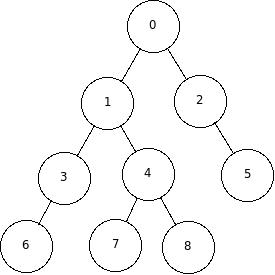
\includegraphics[scale=0.7]{arbre9sommets}
\end{center}
\end{block}
\end{frame}

\begin{frame}
\frametitle{Algorithme lin�aire}
\begin{block}{Exemple}
\begin{center}
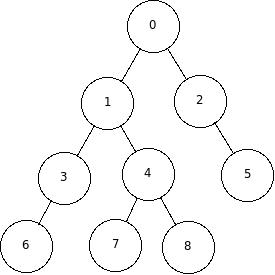
\includegraphics[scale=0.4]{arbre9sommets}\\
couverture : 3
\end{center}
\end{block}
\end{frame}

\begin{frame}
\frametitle{Algorithme lin�aire}
\begin{block}{Exemple}
\begin{center}
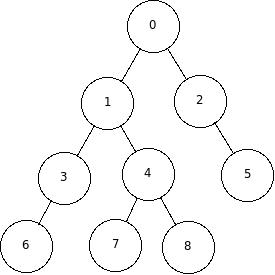
\includegraphics[scale=0.4]{arbre9sommets}\\
couverture : 3 - 4
\end{center}
\end{block}
\end{frame}

\begin{frame}
\frametitle{Algorithme lin�aire}
\begin{block}{Exemple}
\begin{center}
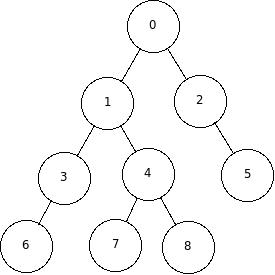
\includegraphics[scale=0.4]{arbre9sommets}\\
couverture : 3 - 4 - 2
\end{center}
\end{block}
\end{frame}

\begin{frame}
\frametitle{Algorithme lin�aire}
\begin{block}{Exemple}
\begin{center}
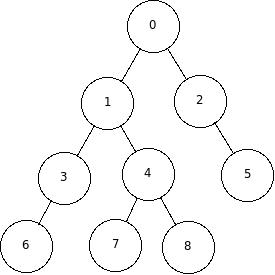
\includegraphics[scale=0.4]{arbre9sommets}\\
couverture : 3 - 4 - 2 - 0
\end{center}
\end{block}
\end{frame}

\begin{frame}[fragile]
\frametitle{Algorithme lin�aire}
\begin{block}{Fichier gengraph}
\begin{verbatim}
0-1 0-2 1-3 1-4 3-6 4-7 4-8 2-5
\end{verbatim}
\end{block}

\begin{block}{R�sultat}
\begin{verbatim}
0 2 3 4
\end{verbatim}
\end{block}
\end{frame}
